\documentclass[xcolor=svgnames,t]{beamer}

% ====== Colores y tema (según tu plantilla) ======
\definecolor{myuniversity}{RGB}{0,60,113}
\definecolor{internationalorange}{RGB}{231,93,42}
\definecolor{dodgerblue}{RGB}{0,60,113}

\usetheme{Madrid}
\usecolortheme[named=myuniversity]{structure}
\useoutertheme{infolines}

% ====== Paquetes mínimos ======
\usepackage[utf8]{inputenc} % si compilas con pdfLaTeX
\usepackage{booktabs,comment}
\usepackage[absolute,overlay]{textpos}
\usepackage{amsmath}
\usepackage[makeroom]{cancel}
\usepackage{tikz}
\usetikzlibrary{calc,positioning}
\usepackage{graphicx}
\usepackage{ragged2e}
\usepackage{hyperref}
\usepackage{fontawesome5}
%\usepackage[colorlinks=true, urlcolor=blue]{hyperref}

% ====== Estilo de encabezados/pie ======
\setbeamercolor{title in head/foot}{bg=internationalorange}
\setbeamercolor{author in head/foot}{bg=dodgerblue}
\setbeamertemplate{caption}[numbered]
\setbeamertemplate{navigation symbols}{}

% ====== Título ======
\title[Historia de la IA]{Módulo 3: Fundamentos del Prompt Engineering}

\author[Diego Menares]{Diego Menares}
\institute[Microdatos FEN]{Microdatos\\Universidad de Chile}
\date{\today}
%\titlegraphic{\includegraphics[height=2.2cm]{figs/logo.png}} % Reemplaza por tu logo
%\logo{\includegraphics[height=0.9cm]{figs/logo.png}}

% ====== Número de diapositivas en el pie ======
\addtobeamertemplate{navigation symbols}{}{\hspace{1em}\insertframenumber/\inserttotalframenumber}

% ====== Helpers visuales ======
\newcommand{\tightitem}{\itemsep4pt\parskip0pt\parsep0pt}
\newcommand{\framenote}[1]{\vspace{2mm}{\footnotesize\color{gray}#1}}

\begin{document}

% ====== Portada ======

\begin{frame}
  \titlepage
  \begin{center}
    
\includegraphics[height=1cm]{figs/FEN_CMD-EDContinua_original.png}
  \end{center}
\end{frame}

% ====== Índice ======

% ====== 0. Índice ======
\begin{frame}{Contenido}
\justifying
\begin{itemize}\tightitem
  \item Fundamentos del \textbf{Prompt Engineering}
  \item Naturaleza y propósito
  \item Principios clave
  \item Estructura recomendada
  \item Valor en programación (Python)
  \item \textbf{Sesgos} en LLM y cómo usarlos a favor
  \item Tipos de prompt (0/1/few-shot, CoT, persona, refine, etc.)
  \item Recomendaciones prácticas y referencias
\end{itemize}


\begin{textblock*}{4cm}(9.5cm,8.0cm)
  
\includegraphics[width=3cm]{FEN_CMD-EDContinua_original.png}
\end{textblock*}
\end{frame}

% ====== Lámina: Fundamentos del Prompt Engineering ======
\begin{frame}{Fundamentos del Prompt Engineering}
\justifying

\begin{columns}[T,totalwidth=\textwidth]
% ---- Columna texto (mantiene el texto íntegro) ----
\column{0.64\textwidth}
El \textit{prompt engineering} es la disciplina que diseña y redacta de forma deliberada las instrucciones que se dan a un modelo de lenguaje (LLM) para guiarlo hacia una salida específica y de calidad. Aunque un LLM como ChatGPT se basa en técnicas de predicción de texto, su comportamiento puede moldearse significativamente si el \textit{prompt} está bien concebido. Es, en esencia, la interfaz de diseño entre la \textbf{intención humana} y la \textbf{respuesta generada por la IA}.

% ---- Columna diagrama TikZ ----
\column{0.36\textwidth}
\begin{center}
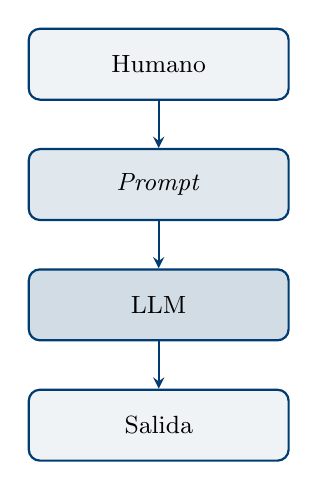
\begin{tikzpicture}[node distance=6mm, >=stealth, thick,
  every node/.style={font=\small},
  box/.style={draw=myuniversity, rounded corners, align=center, inner sep=4pt, minimum width=3.3cm, minimum height=0.9cm}]

\node[box, fill=myuniversity!6] (human) {Humano};
\node[box, fill=myuniversity!12, below=of human] (prompt) {\textit{Prompt}};
\node[box, fill=myuniversity!18, below=of prompt] (llm) {LLM};
\node[box, fill=myuniversity!6, below=of llm] (out) {Salida};

\draw[->,myuniversity] (human) -- (prompt);
\draw[->,myuniversity] (prompt) -- (llm);
\draw[->,myuniversity] (llm) -- (out);

\end{tikzpicture}

\end{center}

\end{columns}



\end{frame}

% ====== Lámina: 1. Naturaleza y propósito ======
\begin{frame}{1. Naturaleza y propósito}
\justifying
Los LLM funcionan como motores de autocompletado extremadamente sofisticados: predicen el siguiente \textit{token} en función del contexto dado. Por eso, la forma en que formulamos la entrada determina:

\begin{itemize}\tightitem
  \item \textbf{Relevancia de la respuesta:} un \textit{prompt} claro reduce ambigüedades.
  \item \textbf{Precisión técnica:} en programación, puede marcar la diferencia entre un código ejecutable y uno con errores.
  \item \textbf{Eficiencia del desarrollo:} un buen \textit{prompt} evita iteraciones innecesarias.
\end{itemize}

\justifying
El objetivo central del \textit{prompt engineering} es \textbf{traducir un problema humano en un conjunto de instrucciones que el modelo pueda interpretar de forma predecible}, para que su salida sea útil y verificable.
\end{frame}


% ====== Lámina: 2. Principios clave ======
\begin{frame}{2. Principios clave}
\justifying
La práctica efectiva del \textit{prompt engineering} se apoya en varios principios:

\begin{itemize}\tightitem
  \item \textbf{Claridad y especificidad:} expresar el problema en términos concretos, evitando ambigüedades.
  \item \textbf{Contexto suficiente:} proporcionar información de entorno (lenguaje de programación, restricciones de datos, objetivo final) para que el modelo entienda el escenario.
  \item \textbf{Orientación al objetivo:} el \textit{prompt} no solo pregunta, sino que define qué forma debe tener la respuesta: un bloque de código, una explicación paso a paso o un archivo en un formato determinado.
  \item \textbf{Iteración y refinamiento:} el \textit{prompt} se mejora de manera progresiva, analizando las salidas y ajustando las instrucciones para alcanzar el resultado deseado.
\end{itemize}

\justifying
Estos principios hacen que el diseño de \textit{prompts} sea un \textbf{proceso de ingeniería}, más que un simple arte de redactar preguntas.
\end{frame}

% ====== Lámina: 3. Estructura recomendada ======
\begin{frame}{3. Estructura recomendada}
\justifying
[Berryman y Ziegler, 2024] proponen visualizar el \textit{prompt} como un documento técnico con partes definidas, adaptables a cada tarea:

\begin{enumerate}\tightitem
  \item \textbf{Contexto:} breve descripción del problema, del entorno o de los datos relevantes.
  \item \textbf{Instrucción principal:} lo que se quiere que el modelo produzca, en forma de acción concreta.
  \item \textbf{Criterios de salida:} formato esperado (código en Python, JSON, tabla, explicación textual).
  \item \textbf{Condiciones o restricciones:} por ejemplo, uso de librerías estándar, límites de tiempo o estilo de programación.
\end{enumerate}

\justifying
Una estructura así no solo mejora la \textbf{calidad de la respuesta}, sino que también facilita su \textbf{reproducibilidad} e \textbf{integración} en flujos de trabajo de desarrollo.
\end{frame}


% ====== Lámina: 4. Valor en programación ======
\begin{frame}{4. Valor en programación}
\justifying

\begin{columns}[T,totalwidth=\textwidth]
% ---- Columna izquierda: texto íntegro ----
\column{0.63\textwidth}
En el contexto de Python y del desarrollo de software, estos fundamentos se convierten en una \textbf{herramienta estratégica}:

\vspace{0.5em}
\begin{itemize}
  \item Permiten obtener \textbf{código más seguro y mantenible} desde el primer intento.
  \item Facilitan la \textbf{automatización de tareas repetitivas} sin necesidad de reentrenar modelos.
  \item Favorecen la \textbf{colaboración humano–IA}, transformando al LLM en un verdadero asistente de programación.
\end{itemize}


% ---- Columna derecha: imagen de código ----
\column{0.37\textwidth}
\vspace{2.5em}
\begin{center}
  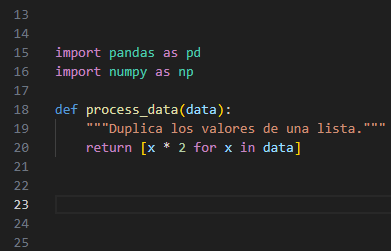
\includegraphics[width=4.5cm]{figs/example_python.png}
  \framenote{Ejemplo código de python}
\end{center}

\end{columns}

\end{frame}

% ====== Lámina: Sesgos y aprovechamiento ======
\begin{frame}{Sesgos en los Modelos de Lenguaje y su Aprovechamiento en el Diseño de \textit{Prompts}}

Los modelos de lenguaje no son neutrales. Al entrenarse en enormes volúmenes de texto para predecir el siguiente \textit{token} con máxima probabilidad, desarrollan patrones de respuesta que llamamos \textbf{sesgos}. Lejos de ser solo un problema, estos sesgos pueden \textbf{aprovecharse de forma consciente en el \textit{prompt engineering}} [Berryman y Ziegler, 2024].

\medskip
\medskip
Comprender por qué surgen, a nivel matemático, permite diseñar \textit{prompts} que los utilicen en nuestro favor.

\begin{textblock*}{4cm}(9.5cm,8.0cm)
  
\includegraphics[width=3cm]{FEN_CMD-EDContinua_original.png}
\end{textblock*}

\end{frame}


% 4.1
\begin{frame}{4.1 Efecto de posición: \textit{primacy} y \textit{recency}}
\textbf{Qué es:}\\
La información situada al inicio del \textit{prompt} influye más en el formato y el tono, mientras que lo del final impacta más en el contenido sustantivo. La parte central suele perder fuerza, fenómeno conocido como “\textit{Valley of Meh}”.

\medskip
\textbf{Génesis técnica:}\\
Los \textit{Transformers} utilizan mecanismos de \textit{auto-atención} con codificación posicional. Durante el entrenamiento, las cabeceras de atención tienden a asignar más atención a los tokens de los extremos, y la entropía cruzada premia la predicción eficiente del siguiente \textit{token}. Como resultado, el modelo recuerda mejor el principio y el final de la secuencia, mientras la información intermedia queda atenuada.

\medskip
\textbf{Uso estratégico:}\\
Colocar al principio las instrucciones de estilo (por ejemplo, “Sigue PEP8 y comenta cada función”) y al final los datos clave o la pregunta central para que el modelo los priorice.
\end{frame}

% ====== Lámina: 4.2 Sesgo de anclaje ======
\begin{frame}{4.2 Sesgo de anclaje}
\justifying
\textbf{Qué es:}\\
Tendencia a dar peso desproporcionado a la primera pista o contexto recibido.

\medskip
\textbf{Génesis técnica:}\\
En la \textit{auto-atención}, los primeros tokens suelen servir para establecer la representación de contexto. Como el modelo predice token a token, las primeras señales condicionan la distribución de probabilidades de todo el resto, generando un “efecto arrastre” en el razonamiento.

\medskip
\textbf{Uso estratégico:}\\
Emplear un “ancla” deliberada:

\medskip
\textit{“Actúa como revisor senior de código Python y optimiza la eficiencia del siguiente script.”}\\
De esta manera se fija de inicio la perspectiva que el modelo mantendrá.
\end{frame}

% ====== Lámina: 4.3 Sesgo de confirmación ======
\begin{frame}{4.3 Sesgo de confirmación}
\justifying
\textbf{Qué es:}\\
El modelo tiende a reforzar la hipótesis implícita en la pregunta, en lugar de cuestionarla.

\medskip
\textbf{Génesis técnica:}\\
El objetivo de entrenamiento minimiza la pérdida buscando la continuación más plausible dado el contexto. Si el \textit{prompt} insinúa una respuesta, la distribución de probabilidad se concentra en tokens que la confirmen; “contradecir” el contexto tiene menor probabilidad.

\medskip
\textbf{Uso estratégico:}\\
Presentar la hipótesis y luego pedir crítica:

\medskip
\textit{“Mi algoritmo burbuja es eficiente. Examina y explica por qué esta afirmación podría ser incorrecta.”}\\
Así se induce al modelo a primero confirmar y luego, por indicación explícita, buscar contraargumentos.
\end{frame}

% ====== Lámina: 4.4 Sesgo de disponibilidad o popularidad ======
\begin{frame}{4.4 Sesgo de disponibilidad o popularidad}
\justifying
\textbf{Qué es:}\\
Favorece soluciones o ejemplos frecuentes en los datos de entrenamiento.

\medskip
\textbf{Génesis técnica:}\\
El entrenamiento en \textit{corpora} masivos pondera de forma natural las secuencias más repetidas, ya que éstas tienen mayor probabilidad de aparición y menor pérdida en la predicción. El modelo “prefiere” patrones comunes porque estadísticamente son más seguros.

\medskip
\textbf{Uso estratégico:}\\
Si se busca un estándar conocido:

\medskip
\textit{“Proporciona la forma más común de conectar Python con una base de datos PostgreSQL.”}

\medskip
Y si se quieren alternativas, se debe pedir explícitamente:

\medskip
\textit{“Propón una opción menos frecuente o más innovadora”.}
\end{frame}

% ====== Lámina: 4.5 Efecto halo ======
\begin{frame}{4.5 Efecto halo}
\justifying
\textbf{Qué es:}\\
Tras una primera respuesta convincente, los usuarios tienden a confiar ciegamente en las siguientes.

\medskip
\textbf{Génesis técnica:}\\
No es solo humano: el modelo, al recibir retroalimentación positiva implícita (por ejemplo, continuaciones sin corrección), refuerza patrones de respuesta similares. En paralelo, el sesgo es principalmente del usuario: el tono seguro del modelo genera percepción de autoridad.

\medskip
\textbf{Uso estratégico:}\\
Pedir siempre \textit{auto-revisión}:

\medskip
\textit{“Ahora revisa tu propio código y señala posibles vulnerabilidades de seguridad.”}\\
Se fuerza al modelo a cuestionar su propia salida y se evita caer en confianza ciega.
\end{frame}


% ====== Lámina: Bias-aware prompting ======
\begin{frame}{\textit{Bias-aware prompting}}
\justifying

Esta práctica, propuesta por \textbf{[Berryman y Ziegler, 2024]}, consiste en \textbf{conocer los sesgos y explotarlos conscientemente} para guiar el comportamiento del modelo. 
No se trata de eliminarlos, sino de \textbf{usarlos como palancas de diseño}, siempre validando externamente mediante \textbf{pruebas unitarias}, \textbf{revisión de código} y \textbf{documentación oficial}.


\begin{center}
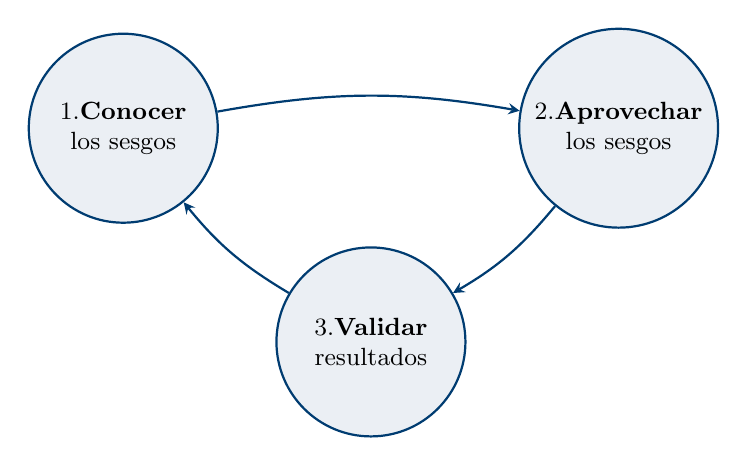
\begin{tikzpicture}[node distance=2.6cm,>=stealth,thick,
  every node/.style={font=\small,align=center},
  box/.style={draw=myuniversity, fill=myuniversity!8, circle, minimum size=2.4cm}]

% Nodos del ciclo
\node[box] (A) {1.\textbf{Conocer}\\los sesgos};
\node[box, right=3.8cm of A] (B) {2.\textbf{Aprovechar}\\los sesgos};

% Punto medio entre A y B
\path let \p1 = (A), \p2 = (B) in coordinate (mid) at ($(\p1)!.5!(\p2)$);

% Nodo inferior centrado
\node[box, below=1.5cm of mid] (C) {3.\textbf{Validar}\\resultados};

% Flechas del ciclo
\draw[->,myuniversity,thick] (A) to[bend left=10] (B);
\draw[->,myuniversity,thick] (B) to[bend left=10] (C);
\draw[->,myuniversity,thick] (C) to[bend left=10] (A);

\end{tikzpicture}
\end{center}

\end{frame}


% ====== Lámina: Resumen de sesgos ======
{
\begin{frame}{Resumen: Sesgos en los Modelos de Lenguaje}
\justifying

\vspace{0.2cm}
\begin{center}
\textcolor{myuniversity}{\large \faBalanceScale\hspace{0.4em} Comprender los sesgos permite diseñar mejores \textit{prompts}}
\end{center}

\vspace{0.5cm}

\begin{columns}[T,totalwidth=\textwidth]
% --- Columna izquierda ---
\column{0.48\textwidth}
\begin{itemize}\tightitem
  \item[\faArrowUp] \textbf{Efecto de posición:} el inicio y el final pesan más que el medio.
  \item[\faAnchor] \textbf{Sesgo de anclaje:} la primera instrucción fija el tono del razonamiento.
  \item[\faSearch] \textbf{Sesgo de confirmación:} el modelo refuerza hipótesis en lugar de cuestionarlas.
\end{itemize}

% --- Columna derecha ---
\column{0.48\textwidth}
\begin{itemize}\tightitem
  \item[\faChartBar] \textbf{Sesgo de disponibilidad:} prefiere ejemplos comunes en los datos.
  \item[\faSun] \textbf{Efecto halo:} respuestas iniciales convincentes generan confianza ciega.
\end{itemize}


\end{columns}

\begin{textblock*}{4cm}(9.5cm,8.0cm)
  
\includegraphics[width=3cm]{FEN_CMD-EDContinua_original.png}
\end{textblock*}

\end{frame}

% ====== Lámina: Tipos de Prompt para Programación en Python ======
\begin{frame}{Tipos de \textit{Prompt} para Programación en Python}
\justifying

\begin{columns}[T,totalwidth=\textwidth]
% ---- Columna izquierda: texto original ----
\column{0.63\textwidth}
\textbf{Contexto:}\\
La calidad del código que generan los modelos de lenguaje depende fuertemente de la forma en que se formula el \textit{prompt}. 

\medskip
Los estudios recientes en ingeniería de \textit{prompts} para programación identifican \textbf{patrones y técnicas} que mejoran la \textbf{precisión}, la \textbf{seguridad} y la \textbf{mantenibilidad} del código generado \textbf{[Della Porta et al., 2025; Tony et al., 2024; Berryman \& Ziegler, 2024]}.



% ---- Columna derecha: visual / apoyo ----
\column{0.37\textwidth}
\begin{center}
% Diagrama con los tres ejes técnicos
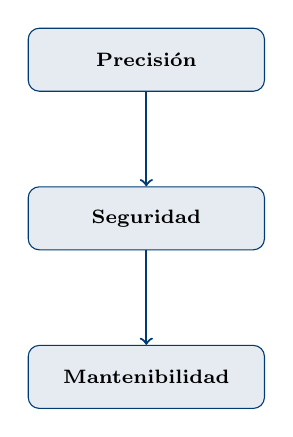
\begin{tikzpicture}[node distance=1.2cm, every node/.style={font=\scriptsize,align=center}]
\node[draw=myuniversity,fill=myuniversity!10,rounded corners,minimum width=3cm,minimum height=0.8cm] (prec) {\textbf{Precisión}};
\node[draw=myuniversity,fill=myuniversity!10,rounded corners,below=of prec,minimum width=3cm,minimum height=0.8cm] (seg) {\textbf{Seguridad}};
\node[draw=myuniversity,fill=myuniversity!10,rounded corners,below=of seg,minimum width=3cm,minimum height=0.8cm] (mant) {\textbf{Mantenibilidad}};
\draw[myuniversity,thick,->] (prec) -- (seg);
\draw[myuniversity,thick,->] (seg) -- (mant);
\end{tikzpicture}
\end{center}
\end{columns}

\end{frame}
% ====== Lámina: 5.1 Zero-Shot Prompting ======
\begin{frame}{5.1 Zero-Shot Prompting}
\justifying
\textbf{Descripción:}\\
El modelo recibe solo la instrucción, sin ejemplos previos.

\medskip
\textbf{Ventajas:}
\begin{itemize}\tightitem
  \item Rápido y directo; ideal para tareas estándar o cuando no hay datos de entrenamiento específicos.
\end{itemize}

\textbf{Desventajas:}
\begin{itemize}\tightitem
  \item Puede generar código incompleto o inseguro si la tarea es compleja.
\end{itemize}

\textbf{Ejemplo en Python:}\\
\textit{“Escribe una función en Python que calcule la mediana de una lista de números.”}

\medskip
\textbf{Uso recomendado:}\\
Tareas simples, utilidades de \textit{scripting}, prototipos rápidos.
\end{frame}

% ====== Lámina: 5.2 One-Shot y Few-Shot Prompting ======
\begin{frame}{5.2 One-Shot y Few-Shot Prompting}
\justifying
\textbf{Descripción:}\\
Se incluyen uno o varios ejemplos de entrada–salida antes de la solicitud principal.

\medskip
\textbf{Beneficio:}\\
El modelo aprende el formato y el estilo deseado a partir de los ejemplos.

\medskip
\textbf{Consideración:}\\
Requiere preparar ejemplos relevantes y bien diseñados.

\medskip
\textbf{Ejemplo (\textit{few-shot}) en Python:}\\
Entrada: \texttt{[1,2,3]} $\rightarrow$ Salida: \texttt{2}\\
Entrada: \texttt{[4,4,5]} $\rightarrow$ Salida: \texttt{4}\\
Ahora: Calcula la mediana de \texttt{[10,2,3,8]}

\medskip
\textbf{Aplicación:}\\
Cuando se necesita un estilo de código consistente (por ejemplo, siguiendo PEP8) o un patrón de arquitectura repetible.
\end{frame}

% ====== Lámina: 5.3 Chain-of-Thought (CoT) ======
\begin{frame}{5.3 Chain-of-Thought (CoT)}
\justifying
\textbf{Descripción:}\\
Se indica explícitamente que el modelo razone paso a paso antes de dar el resultado.

\medskip
\textbf{Fortalezas:}\\
Mejora la lógica en algoritmos complejos; útil para problemas de optimización o estructuras de datos avanzadas.

\medskip
\textbf{Ejemplo en Python:}\\
\textit{“Piensa paso a paso: primero describe el algoritmo para ordenar una lista enlazada y luego escribe el código en Python.”}

\medskip
\textbf{Consejo:}\\
Ideal para \textit{debugging} y para comprender el razonamiento detrás del código generado.
\end{frame}
% ====== Lámina: 5.4 Persona-based Prompting ======
\begin{frame}{5.4 Persona-based Prompting}
\justifying
\textbf{Descripción:}\\
Se asigna un rol específico al modelo para influir en el estilo de la solución.

\medskip
\textbf{Ejemplo:}\\
\textit{“Actúa como un ingeniero senior en Python experto en seguridad. Genera una función que procese datos de usuario evitando inyecciones SQL.”}

\medskip
\textbf{Utilidad:}\\
Asegura que el código cumpla con estándares de seguridad o con un nivel de calidad específico.
\end{frame}

% ====== Lámina: 5.5 Refinement-Based Techniques ======
\begin{frame}{5.5 Refinement-Based Techniques}
\justifying
\textbf{Descripción:}
Orientadas a iterar y mejorar el resultado en ciclos sucesivos \textbf{[Tony et al., 2024; Berryman \& Ziegler, 2024]}.

\medskip
\textbf{a) Recursive Criticism and Improvement (RCI)}\\
El modelo revisa su propio código, identifica errores y los corrige en ciclos sucesivos.

\medskip
\textbf{Ejemplo:}\\
\textit{“Genera un script de Python que haga web \textit{scraping}.\\
Ahora revisa tu respuesta y señala posibles problemas de seguridad.\\
Corrige el código según tu revisión.”}

\medskip
\textbf{b) Self-Refine}\\
Similar a RCI, pero con pasos automáticos de autoevaluación y mejora continua.

\medskip
\textbf{Beneficio:}
Refuerza la calidad y seguridad del código sin intervención constante del usuario.
\end{frame}

% ====== Lámina: 5.6 Progressive Hint Prompting ======
\begin{frame}{5.6 Progressive Hint Prompting}
\justifying
\textbf{Descripción:}\\
El modelo recibe pistas progresivas que lo guían hacia la solución.

\medskip
\textbf{Uso en Python:}\\
Cuando se busca que el modelo construya un algoritmo complejo en etapas, por ejemplo:
\begin{enumerate}\tightitem
  \item Diseñar la estructura de clases.
  \item Implementar los métodos.
  \item Optimizar la eficiencia.
\end{enumerate}

\medskip
\textbf{Ventaja:}\\
Favorece el aprendizaje guiado y la generación de código modular.
\end{frame}


% ====== Lámina: 5.7 Least-to-Most Prompting ======
\begin{frame}{5.7 Least-to-Most Prompting}
\justifying
\textbf{Descripción:}\\
Se comienza resolviendo subtareas simples y se avanza hacia la tarea más compleja.

\medskip
\textbf{Ejemplo:}\\
Primero pedir funciones auxiliares (p. ej., para validar entradas), luego la función principal.

\medskip
\textbf{Beneficio:}\\
Facilita el desarrollo de software modular y \textit{testable}, y reduce la probabilidad de errores en etapas posteriores.
\end{frame}


% ====== Lámina: 5.8 Output Customization / Error Identification ======
\begin{frame}{5.8 Output Customization / Error Identification}
\justifying
\textbf{Descripción:}\\
Patrones donde el \textit{prompt} exige un formato de salida específico (por ejemplo, solo código) o que el modelo detecte y explique errores en su propia respuesta.

\medskip
\textbf{Ejemplo:}\\
\textit{“Escribe únicamente el código Python, sin explicaciones. Luego genera un reporte de errores potenciales en el mismo script.”}

\medskip
\textbf{Aplicación:}\\
Útil para \textit{pipelines} automáticos de verificación de código y para entornos de desarrollo continuo.
\end{frame}

% ====== Lámina: Recomendaciones Prácticas para Python ======
\begin{frame}{Recomendaciones Prácticas para Python}
\justifying

\vspace{0.3em}
\begin{itemize}\tightitem
  \item \textbf{Combina técnicas:} Por ejemplo, inicia con \textit{few-shot} y agrega una fase RCI para reforzar la seguridad del código \textbf{[Tony et al., 2024; Berryman \& Ziegler, 2024]}.
  \item \textbf{Especifica entorno y librerías:} Indica versión de Python, dependencias o \textit{frameworks}.
  \item \textbf{Integra validación automática:} Añade en el \textit{prompt} la instrucción de crear \textit{tests} unitarios para verificar la solución.
\end{itemize}

\begin{beamercolorbox}[rounded=true,wd=\linewidth,sep=4pt]{block body}
\scriptsize
\texttt{\# entorno}\\
\texttt{python=3.11~~pandas=2.2~~pytest=8}
\end{beamercolorbox}

\vspace{0.25cm}

\begin{beamercolorbox}[rounded=true,wd=\linewidth,sep=4pt]{block body}
\scriptsize
\texttt{\# test rápido}\\
\texttt{def test\_suma():}\\
\hspace*{0.8em}\texttt{assert (2+2) == 4}
\end{beamercolorbox}


\end{frame}
% ====== Lámina: Referencias ======
\begin{frame}{Referencias}
\small
\begin{itemize}\tightitem
  \item Berryman, J., \& Ziegler, A. (2024). \textit{Prompt Engineering for LLMs: The Art and Science of Building Large Language Model–Based Applications}. O’Reilly Media.
  \item Della Porta, A., Lambiase, S., \& Palomba, F. (2025). \textit{Do Prompt Patterns Affect Code Quality? A First Empirical Assessment of ChatGPT-Generated Code}. arXiv:2504.13656v1.
  \item Tony, C., Díaz Ferreyra, N. E., Mutas, M., Dhiff, S., \& Scandariato, R. (2024). \textit{Prompting Techniques for Secure Code Generation: A Systematic Investigation}. arXiv:2407.07064v2.
\end{itemize}
\end{frame}


\end{document}